\documentclass[blue]{beamer}

\usepackage[utf8]{inputenc}
\usepackage{default}

%theme split
\usepackage{beamerthemesplit}
%theme shadow
\usepackage{beamerthemeshadow}

\usepackage{amsthm,amssymb,mathrsfs,setspace,pstcol,textcomp,amsmath}
\usepackage{amsmath}
\usepackage{setspace}
\usepackage{epsfig}
\usepackage{color}
\usepackage{geometry}    
\usepackage{graphicx}
\usepackage{graphics}
%\usepackage{comment}
\usepackage{float}
\restylefloat{figure}
%\usepackage[demo]{graphicx}
%\usepackage{floatrow}

%%%%%%%%%%%%%%%%%%%%%%%%%Starting of document %%%%%%%%%%%%%%%%%%%%%%%%%%%%%%%%%%%%%%%%%
\begin{document}

%%%%%%%%%%%%%%%%%%%%%%%%%%%%Title%%%%%%%%%%%%%%%%%%%%%%%%%%%%%%%%%%%%%%%%%%%
\title 
[Discrete Dics Cover Problem
\hspace{0.5cm}
\insertframenumber / \inserttotalframenumber]
{BTP Presentation : \\ Discrete Disc Cover Problem }

%%%%%%%%%%%%%%%%%%%%%%%%%%%%%Author%%%%%%%%%%%%%%%%%%%%%%%%%%%%%%%%%%%%%%%%%%
\author
 [Raj Kamal]
 {Raj Kamal\\
  Indian Institute of Technology, Guwahati\\
  r.kamal@iitg.ernet.in\\
  Under the Guidance of Dr. Gautam K. Das\\
  \date {IIT Guwahati\\
   17 April 2013}}
   
%%%%%%%%%%%%%%%%%%%%%%%%%%%%%%%%%%%%Starting of Frame %%%%%%%%%%%%%%%%%%%%%%%%
   \begin{frame}
 \titlepage
\end{frame}

%%%%%%%%%%%%%%%%%%%%%%New Frame %%%%%%%%%%%%%%%%%%%%%%%%%%%%%%%%%%%%%%%%%%%%%%
\begin{frame}
\frametitle{Introduction}
{\color{red}\textbf{Covering Problem}}
\begin{itemize}
   
    \item Minimization problem
    \item One geometric structure covers another geometric structure with given constraints
    \item How large dimension should be
    \item NP Complete Problem
    \item {\color{blue}{Approximation and Statistical methods}}
   \end{itemize}
  \begin{figure}[H]
% {\caption{A test figure with its caption side by side}\label{fig:test}}
     \caption{Covering with voronio diagram} 
   %  \label{fig:test}
        \centering
           \scalebox{0.25}
          {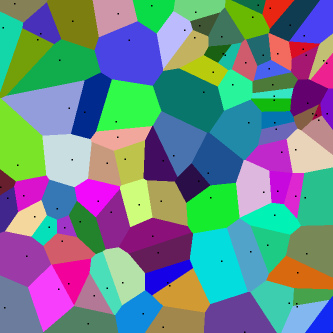
\includegraphics{cover1.png}}
     \end{figure}
\end{frame}

%%%%%%%%%%%%%%%%%%%%%%%%%%%%% New Frame %%%%%%%%%%%%%%%%%%%%%%%%%%%%%%%%%%%%%%%%%%   
\begin{frame}
 \frametitle{Introduction}
 {\color{red}\textbf{Motivation}}
 
 \begin{itemize}
  \item{ Wireless Networking}
    \begin{enumerate}
     \item {\color {blue}{setting wireless gateways}}
     \item {\color {blue}{selecting wireless gateways}}
    \end{enumerate}
  \item Variety of facility location problems
  \item Selecting weather antenna to cover set of cities.
  \item Image processing 
\end{itemize}

\end{frame}

%%%%%%%%%%%%%%%%%%%%%%%%%%%% New frame %%%%%%%%%%%%%%%%%%%%%%%%%%%%%%%%%%%%%%%%%%%
\begin{frame}
 \frametitle{Discrete Disc Cover Problem}
 {\color{red}{\textbf{Description}}} 
 \begin{itemize}
  \item {\color{red}{Red points}} and {\color{blue}{Blue points}} are given in 2D plane.
  \item Circles can be drawn centered at {\color{blue}{blue points}}.
  \item {\color{red}{Red point}} is covered if it lies inside a circle drawn.
  \item {\color{blue}\textbf{Objective}}: Minimum number of blue points such that all red points are covered.
 \end{itemize}

\end{frame}

%%%%%%%%%%%%%%%%%%%%%%%%%%%%%%%%% New Frame %%%%%%%%%%%%%%%%%%%%%%%%%%%%%%%%%%%%%%%%
\begin{frame}
 \frametitle{Discrete Disc Cover Problem}
   \begin{itemize}
   \item {\color{red}{\textbf{Input}}}
     \begin{enumerate}
      \item {\color{red}{$n$ Red Points}}
      \item {\color{blue}{$m$ Blue Points}}
      \item Radius $rad$ to be used of drawing circle 
     \end{enumerate}
    \end{itemize}
    
    \begin{columns}
    \column{0.5 \textwidth}
    {
    \begin{figure}[H]
     \caption{Input}
        \centering
           \scalebox{0.8}
          {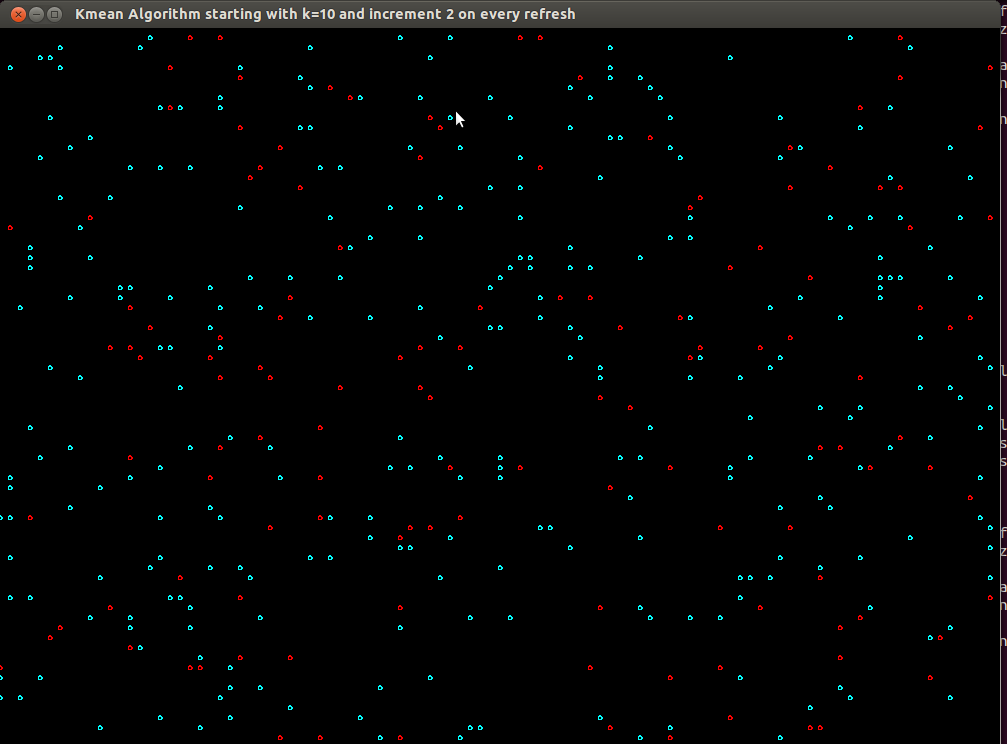
\includegraphics[width=\linewidth]{cover2.png}}
     \end{figure}
    }
    \column{0.5\textwidth}
    {
    \begin{figure}[H]
     \caption{Output}
        \centering
           \scalebox{0.8}
          {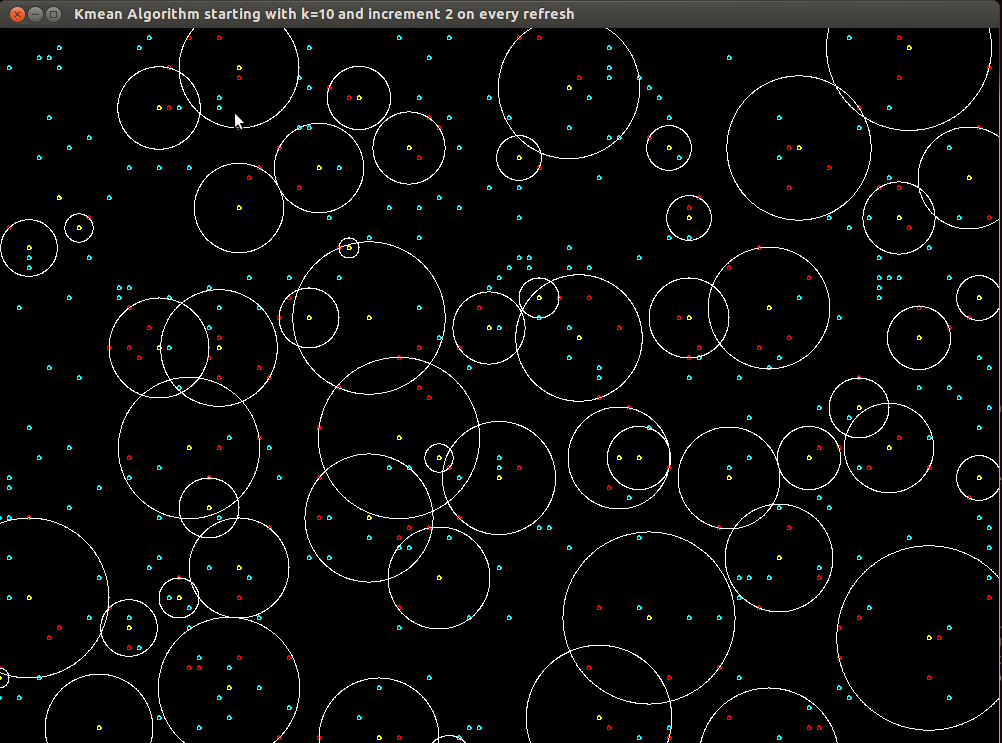
\includegraphics[width=\linewidth]{cover3.png}}
     \end{figure}
    }
     \end{columns}
 \end{frame}
  
%%%%%%%%%%%%%%%%%%%%%%%%%%%%%%%%%%%%%%%%%%%%%%%%New Frame %%%%%%%%%%%%%%%%%%%%%%%%%%%%%%%%%%%% not yet done.....
\begin{frame}
 \frametitle {Related Works}
 \begin{columns}
  \column{0.5\textwidth}
 \begin{itemize}
  \item {\color{red}{\textbf{Discrete Unit Disc Cover Problem}}}
   \begin{itemize}
    \item a set $P$ of $n$ points.
    \item a set $D$ of $m$ unit disks.
    \item DUDC problem is finding minimum cardinality subset $D^{\ast}$ covering all the points in $P$.
    \item Geometric property is explored.
    \item Gautam et al.,\cite{GRALB12}
   \end{itemize}
 \end{itemize}
 \column{0.5\textwidth}
  \begin{figure}[H]
     \caption{DUDC Problem}
        \centering
           \scalebox{0.6}
          {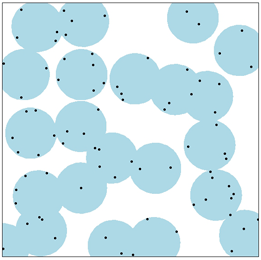
\includegraphics[width=\linewidth]{cover41.png}}
     \end{figure}
     \end{columns}
\end{frame}

%pics.

%%%%%%%%%%%%%%%%%%%%%%%%%%%%%%%%%%%%%%%%%%%%%%% New Frame %%%%%%%%%%%%%%%%%%%%%%%%%%%%%%%%%%%%%%%
\begin{frame}
 \frametitle{Related Works }
 \begin{itemize}
  \item {\color{red}{\textbf{Minimum geometric disk cover}}}  [\cite{T91}, \cite{DW85}].
   \begin{itemize}
    \item set of $n$ points are given
    \item  find unit disk of minimum cardinality whose union covers the points 
     \item  disk centers are not restricted to the set but can be arbitrary points from the plane.
   \end{itemize}
  \item {\color{red}{ \textbf{Discrete K centers }}}
   \begin{itemize}
     \item two sets of points $P$ and $Q$ in two dimensional plane and an integer $K$.
     \item find a set of $K$ disks centered on points in $P$ whose union covers
            $Q$ such that the radius of the largest disk is minimized
   \end{itemize}
   \end{itemize}
  \end{frame}  

%%%%%%%%%%%%%%%%%%%%%%%%%%%%%%%%%%%%%%%%%%%%%%%%%% New Frame %%%%%%%%%%%%%%%%%%%%%%%%%%%%%%%%%%%%%%%%not yet doe......
\begin{frame}
 \frametitle{Related Works}
 \begin{columns}
  \column{0.4 \textwidth}
    \begin{itemize}
    \item Covering with Convex structure. \cite{GSSB}.
    \item Voronoi Diagram are used.
    \end{itemize}
    
    \column{0.6 \textwidth}
     \begin{figure}[H]
     \caption{Voronoi Diagram}
        \centering
           \scalebox{0.6}
          {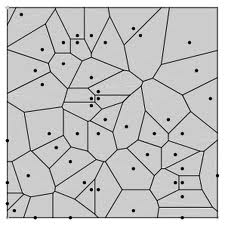
\includegraphics[width=\linewidth]{cover40.png}}
     \end{figure}
 \end{columns}

\end{frame}

%%%%%%%%%%%%%%%%%%%%%%%%%%%%%%%%%%%%%%%%%%%%%%%%%%%%%New Frame %%%%%%%%%%%%%%%%%%%%%%%%%%%%%%%%%%%%
\begin{frame}
 \frametitle{Feasibility}
  \begin{itemize}
  \item {\color{red}\textbf{{Input}}}
  \begin{enumerate}
      \item set $R$ of $n$ {\color{red}{Red Points}}
      \item set $B$ of $m$ {\color{blue} {Blue Points}}
      \item Radius $rad$ to be used of drawing circle
  \end{enumerate}
 \item {\color{red}\textbf{{Feasibility}}}
 \begin{enumerate}
  \item Select a {\color{red}{red point.}}
  \item Find distance with every {\color{blue}{blue point}}
  \item Any distance $<$ rad, the {\color{red}{red point}} can be covered
  \item Repeat the process for all {\color{red}{red point}}
  \item All {\color{red}{red point}} are covered, feasible otherwise not.
 \end{enumerate}
 \end{itemize}
 \end{frame}

%%%%%%%%%%%%%%%%%%%%%%%%%%%%%%%%%%%%%%%%%%%%%%%%)%% New Frame %%%%%%%%%%%%%%%%%%%%%%%%%%%%%%%%%%%%%%%%%%
\begin{frame}
 \frametitle{Algorithm}
  {\color{red}{\textbf{Cluster based approach}}}
  \begin{itemize}
    \item {\textbf{K Mean Continuous Version}}
      \begin{itemize}
         \item {\color{blue}{It is similar to standard K Mean algorithm}} 
         \item {\color{blue}{Continuous Case}}
      \end{itemize}
    \item {\textbf{K Mean Discrete Version}}
      \begin{itemize}
        \item {\color{blue}{Modified K Mean Algorithm}} 
         \item {\color{blue}{Discrete Case}}
       \end{itemize}
   \end{itemize}
\end{frame}
%%%%%%%%%%%%%%%%%%%%%%%%%%%%%%%%%%%%%%%%%%%%%%%%%%%%New Frame %%%%%%%%%%%%%%%%%%%%%%%%%%%%%%%%%%%%%%%%%%%%%
\begin{frame}
 \frametitle{K Mean Continuous Version}
 {\color{red}{\textbf {Input}}}
  \begin{enumerate}
      \item $n$ {\color{red}{Red Points}}
      \item $m$ {\color{blue}{Blue Points}}
      \item Radius $rad$ 
  \end{enumerate}
 {\color{red}{\textbf{Preprocessing assuming conditions are feasible}}}
 \begin{itemize}
  \item Create set of {\color{red}{red}} and {\color{blue}{blue}} points, each element has property 
   \begin{enumerate}
    \item Coordinates
    \item Cover
  \end{enumerate}
 \end{itemize}
\end{frame}

%%%%%%%%%%%%%%%%%%%%%%%%%%%%%%%%%%%%%%%%%%%%%%% New Frame %%%%%%%%%%%%%%%%%%%%%%%%%%%%%%%%%%%%%%%%%%%%%%%
\begin{frame}
\frametitle{K Mean Continuous Version}
\begin{columns}
 
\column{0.5 \textwidth}
 \begin{itemize}
  \item Fix K
  \item Select K randomly {\color{blue}{blue points}}.
  \item {\color{red}\textbf{{Create K cluster.}}}
    \begin{enumerate}
     \item Cluster head
     \item set of Red points
     \item size
     \item radius
    \end{enumerate}
\end{itemize}
\column{0.5 \textwidth}
 \begin{figure}[H]
     \caption{cluster Example }
       % \centering
           \scalebox{0.8}
          {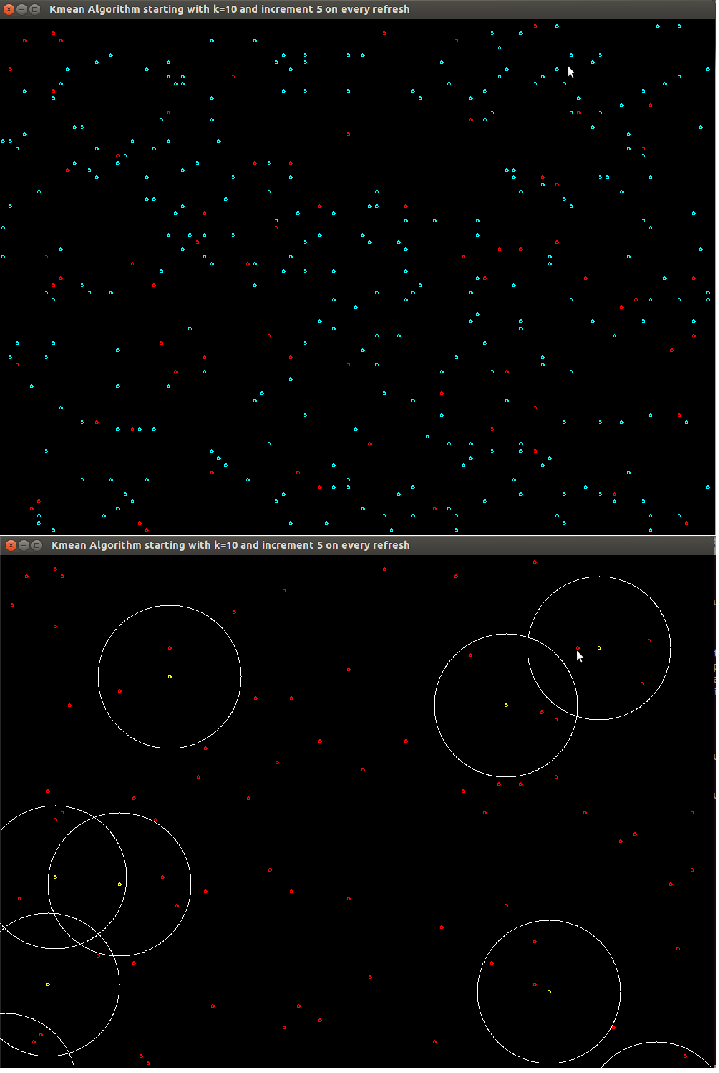
\includegraphics[width=\linewidth ,height=2.6in]{cover15a.png}}
     \end{figure}
 \end{columns}    
{\color{red}{\textbf{Only those red points are in the cluster whose distance from head is less than rad and are covered}}}
\end{frame}

%%%%%%%%%%%%%%%%%%%%%%%%%%%%%%%%%%%%%%%%%%%%%New Frame %%%%%%%%%%%%%%%%%%%%%%%%%%%%%%%%%%%%%%%%%%%%%%%%%%
\begin{frame}
 \frametitle{K Mean Continuous Version}
 \begin{columns}
 \column{0.5 \textwidth}  
 \begin{itemize}
  \item {\color{red}{\textbf{Change Cluster Head}}}
      \begin{enumerate}
       \item We centroid of all {\color{red}{red points}} in set
       \item we change the Cluster head to the centroid
       \item We calculate the difference
      \end{enumerate}
  \item We calculate the $max_diff$ as maximum of difference
  \item If {\color{red}{max$\_$diff $>$ tolerance}} repeat.
  \item We remove unfavorable cluster head.
  \end{itemize}
  \column{0.5 \textwidth}
  \begin{figure}[H]
     \caption{Convergence}
        %\centering
           \scalebox{0.8}
          {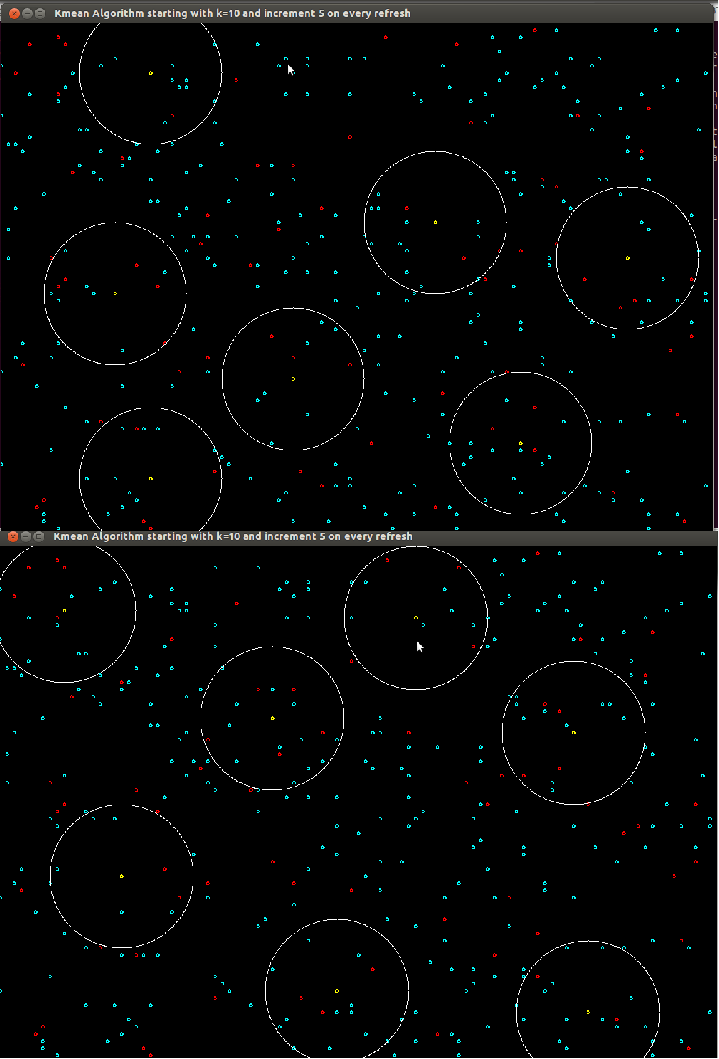
\includegraphics[width=\linewidth, height =2.7in]{cover16a.png}}
     \end{figure}
     \end{columns}
\end{frame}



%%%%%%%%%%%%%%%%%%%%%%%%%%%%%%%%%%%%%%%%%%%%%%%%%% New Frame %%%%%%%%%%%%%%%%%%%%%%%%%%%%%%%%%%%%%%%%%%%%%%%%
\begin{frame}
 \frametitle{K Mean Continuous Version}
 \begin{itemize}
  \item We then check whether all red points are covered or not.
  \item if not then K is incremented and  {\color{red}{create cluster}} and {\color{red}{change cluster}} is repeated.
  \item We have the cover according to original K mean algorithm
  \item Cluster head may not coincide with blue point
  \item We then find nearest {\color{blue}{blue point}} to cluster head and create cluster.
 \end{itemize}
 %%pic of the cover stepss.
\end{frame}

%%%%%%%%%%%%%%%%%%%%%%%%%%%%%%%%%%%%%%%%%%%%%%%%%New Frame %%%%%%%%%%%%%%%%%%%%%%%%%%%%%%%%%%%%%%%%%%%%%%%%%%%%
\begin{frame}
 \frametitle{K Mean Continuous Version}
 \begin{columns}
 \column{0.5 \textwidth} 
 \begin{itemize}
  \item We eliminate unfavorable {\color{blue}{blue points}}.
  \item We cover remaining {\color{red}{red points}} 
 
 \end{itemize}
 \column{0.5 \textwidth}
 \begin{figure}[H]
     \caption{Cluster Example with 100 red point, 400 blue point K=48 }
        \centering
           \scalebox{0.9}
          {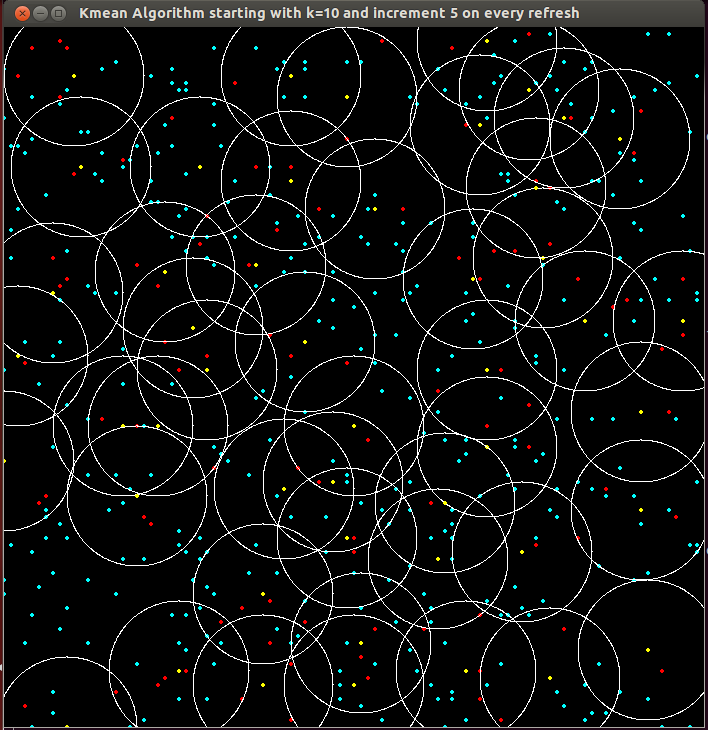
\includegraphics[width=\linewidth ,height =2.0in]{cover28a.png}}
     \end{figure}
 \end{columns}
 {\color{red}\textbf{{Hence cover is obtained.}}}
\end{frame}


 
%%%%%%%%%%%%%%%%%%%%%%%%%%%%%%%%%%%%%%%%%%%%%%%%% New Frame %%%%%%%%%%%%%%%%%%%%%%%%%%%%%%%%%%%%%%%%%%%%%%%
%% lemma and proof
\begin{frame}
 \frametitle{K Mean Continuous Version}
 {\color{red}{\textbf{Lemma}}}: {\color{blue}{Algorithm Converges in every feasible condition.}}
 \begin{itemize}
  \item We show that the maximum radii of the cluster decreases or remains same.
  \item Radius is changed while change in cluster head.
  \item New cluster head is nearest to previous cluster head.
  \item New point may come and some may go out.
  \item New point that has come must have lesser radii than previous maximum. 
  \item Old point goes to new cluster which has lesser radii.
  \item Hence in all cases maximum radius decreases or remains same.
  \item Number of {\color{red}{red points}} are fixed .
  \end{itemize}
\end{frame}


%%%%%%%%%%%%%%%%%%%%%%%%%%%%%%%%%%%%%%%%%%%%%%%%%New Frame %%%%%%%%%%%%%%%%%%%%%%%%%%%%%%%%%%%%%%%%%%%%%%%%%
\begin{frame}
 \frametitle{K Mean Continuous Version}
 {\color{red}{\textbf{Lemma}}}: {\color{blue}{Algorithm will find cover.}}
 \begin{itemize}
  \item Above lemma ensure that the algorithm will converge.
  \item Converged but than all the {\color{red}{red point}} might not covered.
  \item Increase the K and repeat.
  \item At some point we will be able to find cover due to feasibility case.
  \item hence we will be able to get the cover.
 \end{itemize}
\end{frame}

%%%%%%%%%%%%%%%%%%%%%%%%%%%%%%%%%%%%%%%%%%%%%%%%%% NEw Frame %%%%%%%%%%%%%%%%%%%%%%%%%%%%%%%%%%%%%%%%%%%%%%%%
\begin{frame}
 \frametitle{K Mean Continuous Version}
 
  {\color{red}{\textbf{ We obtain the following observations}}}
  \tiny
  \begin{table}[H]
  \centering
  \caption{Convergence with 100 red points and 400 blue points}
  \begin{tabular}{||l|c|c||} \hline
   K    & {\color{blue}{Actual Cluster size}} & {\color{blue}{Red Points Covered}}\\ \hline
   10   & 9                   & {\color{red}{34}}                 \\  \hline
   15   & 14                  & {\color{red}{57}}                  \\  \hline
   20   & 20                  & {\color{red}{81}}                  \\  \hline
   25   & 25                  & {\color{red}{85}}                  \\  \hline
   30   & 27                  & {\color{red}{87}}                  \\   \hline
   35   & 31                  & {\color{red}{92}}                  \\  \hline
   40   & 33                  & {\color{red}{93}}                  \\  \hline
   45   & 39                  & {\color{red}{97}}                   \\  \hline
   50   & 41                  & {\color{red}{99}}                   \\  \hline
   55   & 40                  & {\color{red}{98}}                   \\  \hline
   60   & 47                  & {\color{red}{99}}                   \\   \hline
   65   & 43                  & {\color{red}{100}}                    \\ \hline \hline
 \end{tabular}
 \end{table}
\end{frame}




%%%%%%%%%%%%%%%%%%%%%%%%%%%%%%%%%%%%%%%%%%%%%%%%%%New Frame %%%%%%%%%%%%%%%%%%%%%%%%%%%%%%%%%%%%%%%%%%%%%%%%



%%%%%%%%%%%%%%%%%%%%%%%%%%%%%%%%%%%%%%%%%%%%%%%%%%New Frame %%%%%%%%%%%%%%%%%%%%%%%%%%%%%%%%%%%%%%%%%%%%%%
\begin{frame}
 \frametitle{K Mean Discrete Version}
 {\color{red}{\textbf {Input}}}
  \begin{enumerate}
      \item $n$ {\color{red}{Red Points}}
      \item $m$ {\color{blue}{Blue Points}}
      \item Radius $rad$ 
  \end{enumerate}
 {\color{red}{\textbf{Preprocessing assuming conditions are feasible}}}
 \begin{itemize}
  \item We create {\color{red}{red point}} and {\color{blue}{blue point}} set,each element containing  
   \begin{enumerate}
    \item Coordinates
    \item Cover
   \end{enumerate}
 \end{itemize}
{\color{red}{\textbf{Cover in both entity are different}}}.
\end{frame}

%%%%%%%%%%%%%%%%%%%%%%%%%%%%%%%%%%%%%%%%%%%%%%% New Frame %%%%%%%%%%%%%%%%%%%%%%%%%%%%%%%%%%%%%%%%%%%%%%%
\begin{frame}
\frametitle{K Mean Discrete Version}
 \begin{itemize}
  \item We fix K
  \item We select K randomly {\color{blue}{blue points}}.
  \item Create K cluster.\
    \begin{enumerate}
     \item Coordinates of cluster head.
     \item Set containing {\color{red}{red points}}.
     \item Radius
     \item Size
    \end{enumerate}
\end{itemize}
\textbf{Only those {\color{red}{red points}} are in the cluster whose distance from head is less than rad.}
\end{frame}

%%%%%%%%%%%%%%%%%%%%%%%%%%%%%%%%%%%%%%%%%%%%%%%% New Frame %%%%%%%%%%%%%%%%%%%%%%%%%%%%%%%%%%%%%%%%%%%%%%%%%%
\begin{frame}
 \frametitle{K Mean Discrete Version}
  \begin{itemize}
   \item Clusters head are the selected blue points
   \item All Clusters are put in a Cluster Set.
  \end{itemize}
   \begin{figure}[H]
     \caption{Cluster Example with 200 red point, 400 blue point K=11 }
        \centering
           \scalebox{0.4}
          {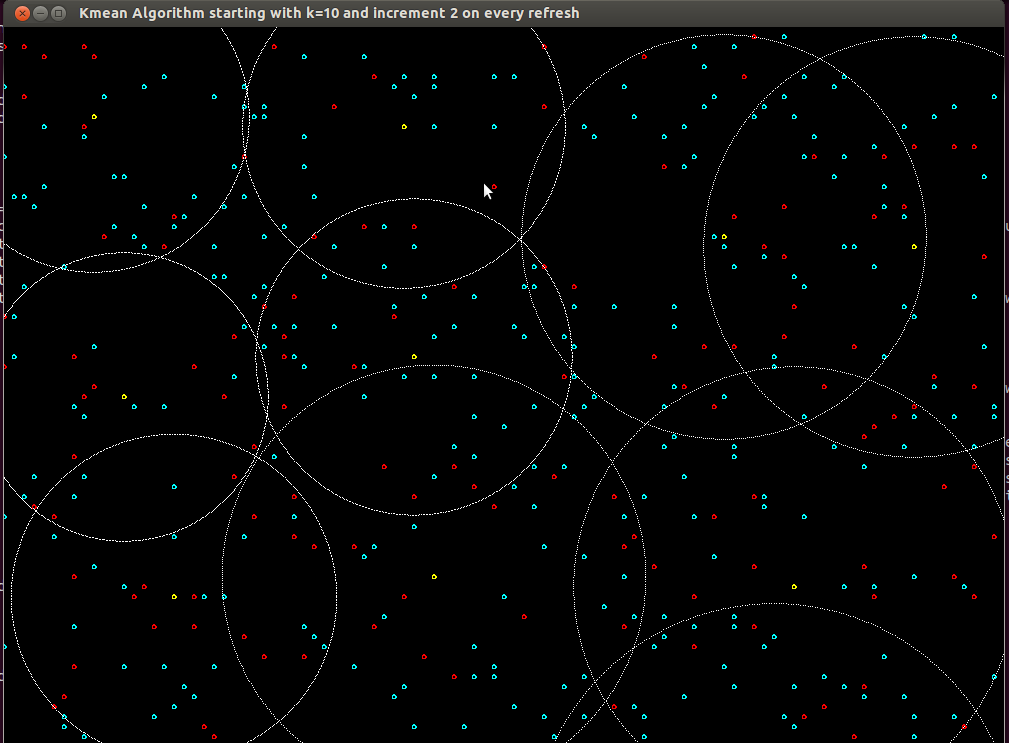
\includegraphics[width=\linewidth, height=3.4 in]{cover4.png}}
     \end{figure}
  \end{frame}

%%%%%%%%%%%%%%%%%%%%%%%%%%%%%%%%%%%%%%%%%%%%%%%%% New Frame %%%%%%%%%%%%%%%%%%%%%%%%%%%%%%%%%%%%%%%%%%%%%%%%%%%%
\begin{frame}
 \frametitle{K Mean Discrete Version}
 \begin{itemize}
  \item We calculate radius of each cluster in the Cluster set
  \item we update the radius of Cluster
  \tiny
  \begin{table}[H]
     \centering
      \vspace{2ex}
          \caption{Radius of each cluster} 
               \begin{tabular}{||l|c|r||} \hline
                     {\color{red}{Cluster}} & {\color{red}{Radius}} & {\color{red}{size}} \\ \hline
                         01 & {\color{blue}{36.2353}} & 24 \\ \hline
                         02 & {\color{blue}{26.4197}} & 16 \\ \hline
                         03 & {\color{blue}{28.3019}} & 11 \\ \hline
                         04 & {\color{blue}{19.2354}} & 14 \\ \hline
                         05 & {\color{blue}{14.0357}} & 3 \\ \hline
                         06 & {\color{blue}{35.4683}} & 24 \\ \hline
                         07 & {\color{blue}{25.4591}} & 23 \\ \hline
                         08 & {\color{blue}{40.6079}} & 40 \\ \hline
                         09 & {\color{blue}{17.8885}} & 9 \\ \hline
                         10 & {\color{blue}{28.0179}} & 15 \\ \hline
                         11 & {\color{blue}{19.2094}} & 11 \\ \hline
                         
                 \end{tabular}
          \end{table}
  \end{itemize}
\end{frame}



%%%%%%%%%%%%%%%%%%%%%%%%%%%%%%%%%%%%%%%%%%%%%%%%%  New Frame %%%%%%%%%%%%%%%%%%%%%%%%%%%%%%%%%%%%%%%%%%%%%%%%%%%
\begin{frame}
\frametitle{ K Mean Discrete Version}
 \begin{itemize}
  \item {\color{red}{\textbf{Change cluster head}}} 
   \begin{itemize}
    \item for each cluster, we find a {\color{blue}{blue point}} nearest to all points.
    \item We update the cluster head to that {\color{blue}{blue point}}, update cover.
   \end{itemize}
   \begin{figure}[H]
             \centering
           \scalebox{0.7}
          {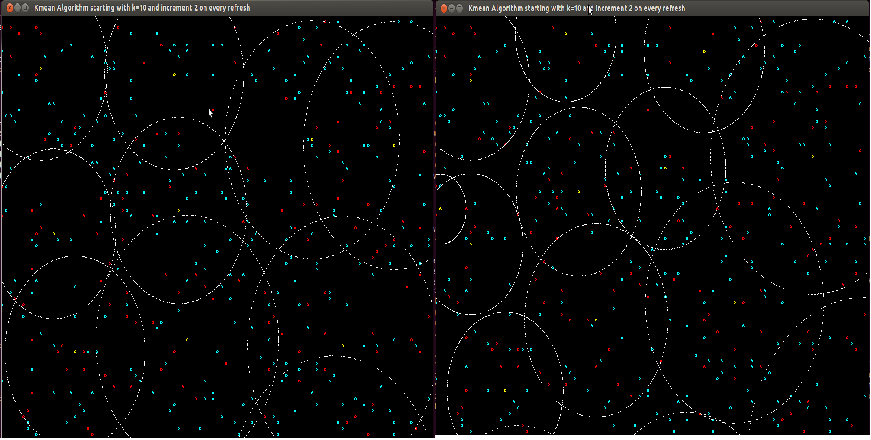
\includegraphics[width=\linewidth,height=1.6in]{cover10.png}}
          \caption{Change in cluster head}
     \end{figure}
     \item {\color{blue}{Calculate the difference b/w old and new cluster head}}
     \item {\color{blue}{Calculate maximum radius.}} 
\end{itemize}
\end{frame}


%%%%%%%%%%%%%%%%%%%%%%%%%%%%%%%%%%%%%%%%%%%%%%%%%%%% New Frame %%%%%%%%%%%%%%%%%%%%%%%%%%%%%%%%%%%%%%%%%%%%%%%%%%%
\begin{frame}
\frametitle{K Mean Discrete Version}
 \begin{itemize}
  \item We calculate maximum difference in change of cluster head
  \item If {\color{red}{maximum difference $>$ tolerance}} then repeat {\color{blue}{the change in cluster}}.
  \item if {\color{red}{maximum radius  $>$ rad}} then increase the K and repeat.
  \begin{figure}[H]
     \caption{Change in K}
        \centering
           \scalebox{0.7}
          {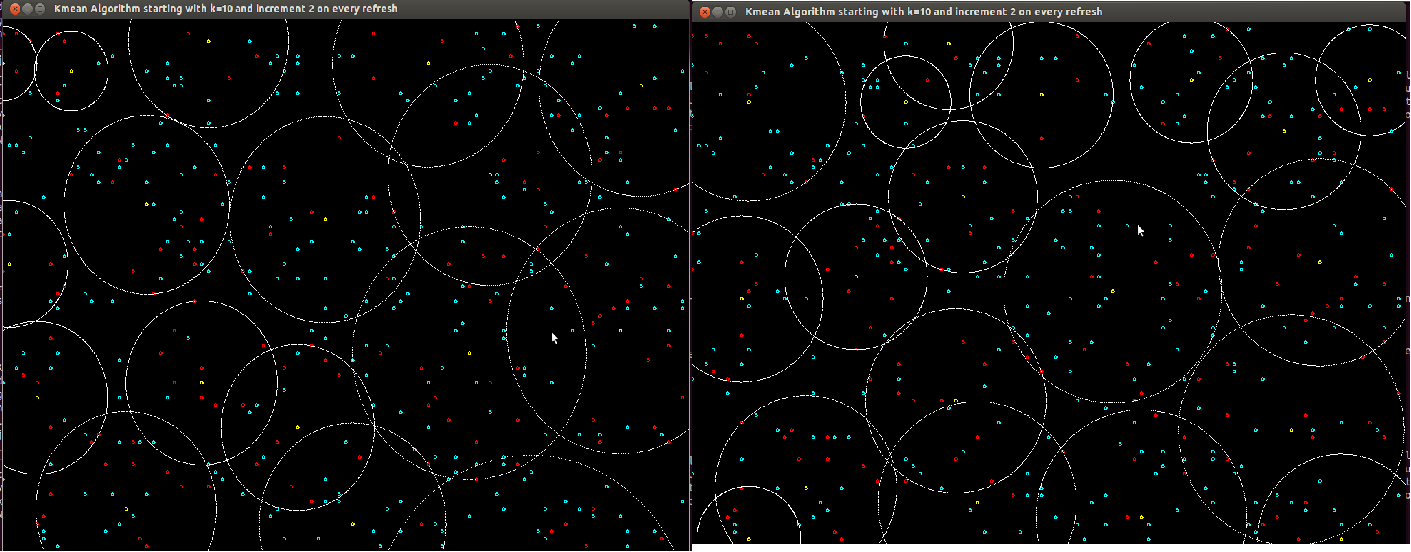
\includegraphics[width=\linewidth]{cover11.png}}
     \end{figure}
   \end{itemize}
\end{frame}

%%%%%%%%%%%%%%%%%%%%%%%%%%%%%%%%%%%%%%%%%%%%%%%%%%%% New Framekjhkhjlkhjlk %%%%%%%%%%%%%%%%%%%%%%%%%%%%%%%%%%%%%%%%%%%%%%%%%%%%%
\begin{frame}
\frametitle{ K Mean Discrete Version}
 \begin{itemize}
  \item Cover remaining {\color{red}{red points}}.
 \end{itemize}
  
  \begin{columns}
   \column{0.5 \textwidth}
   {
  \begin{figure}[H]
     \caption{Final Cover}
        \centering
           \scalebox{1.0}
          {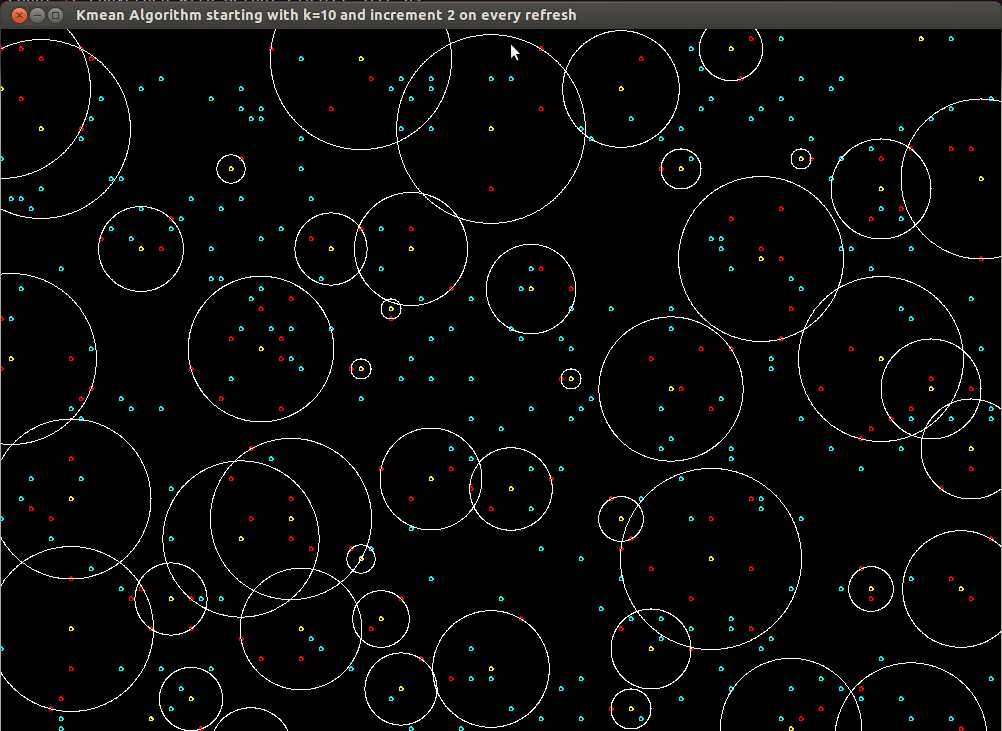
\includegraphics[width=\linewidth, height =1.6 in]{cover9.png}}
     \end{figure}
  }   
  \column{0.5 \textwidth}
  {
  \begin{figure}[H]
  \caption{Process of covering}
        \centering
           \scalebox{1.0}
          {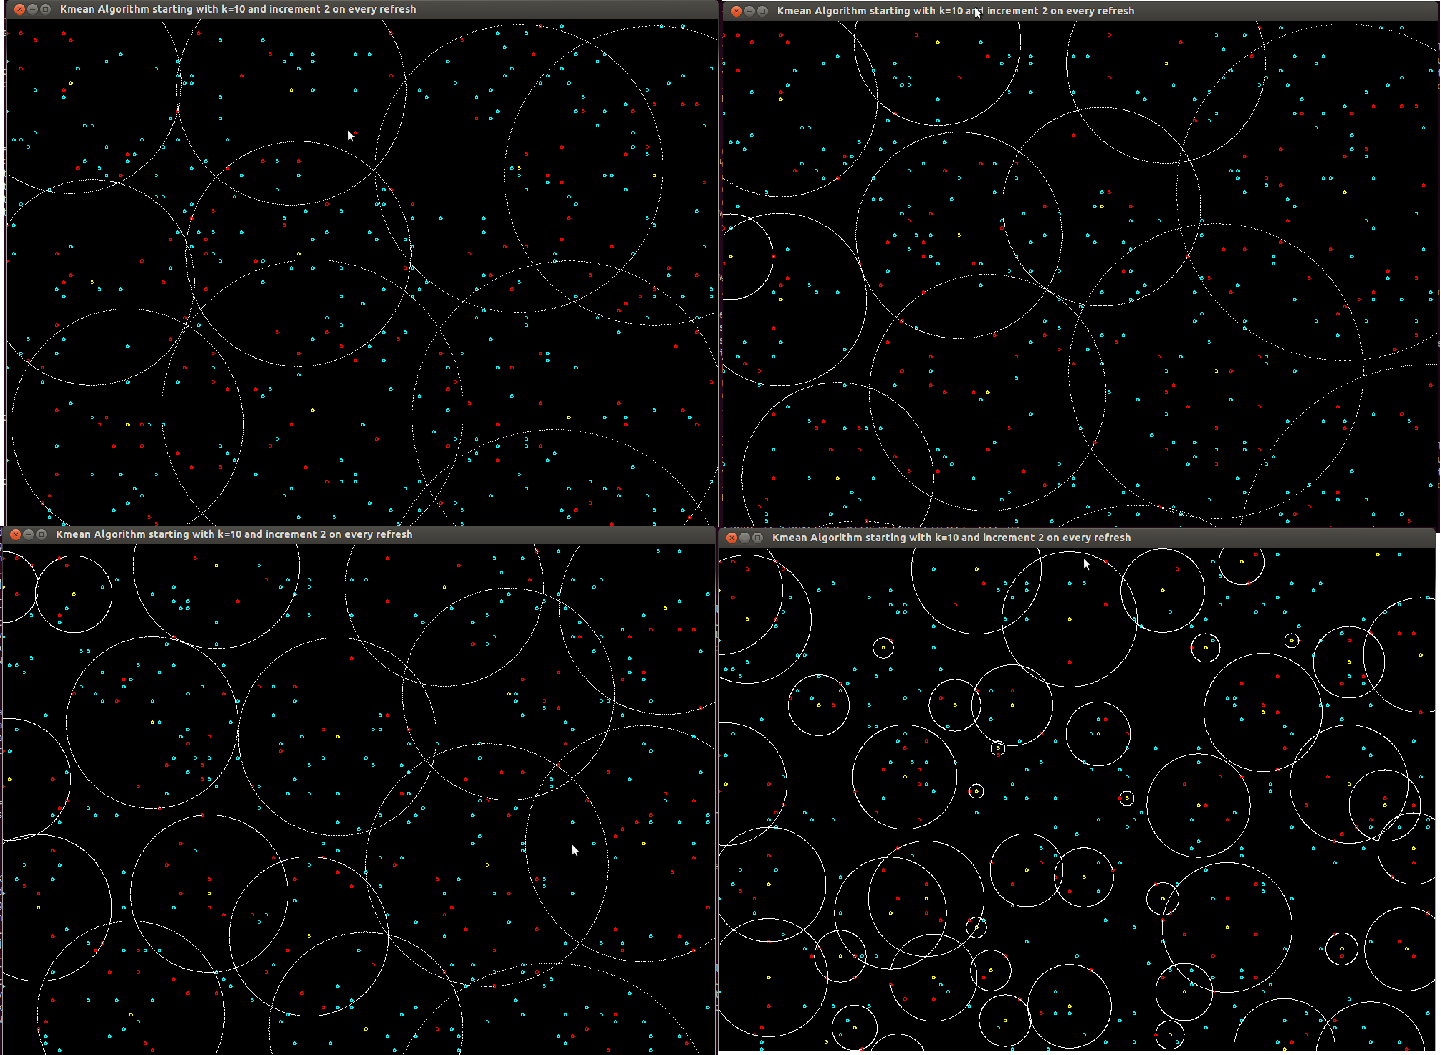
\includegraphics[width=\linewidth, height=1.6in]{cover12.png}}
   \end{figure}
  }
 \end{columns}
\end{frame}

%%%%%%%%%%%%%%%%%%%%%%%%%%%%%%%%%%%%%%%%%%%%%%%%% New Frame %%%%%%%%%%%%%%%%%%%%%%%%%%%%%%%%%%%%%%%%%%%%%%%%%%%%%%%%%%%%
\begin{frame}
 \frametitle{K Mean Discrete Version}
 {\color{red}{\textbf{Lemma}}}:{\color{blue}{The K Mean Discrete Version Algorithm  converges.}}
 \begin{itemize}
  \item The maximum radii of the cluster decreases or remains same.
  \item Radius is changed while change in cluster head
  \item New cluster head is nearest to previous cluster head to the set.
  \item New point may come and some may go out
  \item New point that has come must have lesser radii than previous maximum 
  \item Old point goes to new cluster which has lesser radii.
  \item {\color{blue}{Hence in all cases maximum radius decreases or remains same}}.
  \end{itemize}
\end{frame}


%%%%%%%%%%%%%%%%%%%%%%%%%%%%%%%%%%%%%%%%%%%%%%%%%% New Frame %%%%%%%%%%%%%%%%%%%%%%%%%%%%%%%%%%%%%%%%%%%%%%%%%%%%%%%%%%S
\begin{frame}
 \frametitle{K Mean Discrete Version}
 {\color{red}{\textbf{Lemma}}}:{\color{blue}{K Mean Discrete Version Algorithm finds the cover}}.
 \begin{itemize}
  \item Above lemma ensure that the algorithm will converge.
  \item Converged but than $max\_rad$ is greater than $rad$
  \item Problem is feasible and above lemma
  \item Increase the K and we will be able to find a cover.
  \item Cover remaining
  \item {\color{blue}{Hence we will be able to get the cover}}.
 \end{itemize}
\end{frame}

%%%%%%%%%%%%%%%%%%%%%%%%%%%%%%%%%%%%%%%%%%%%%%% New Frame %%%%%%%%%%%%%%%%%%%%%%%%%%%%%%%%%%%%%%%%%%%%%%%%%%%%%%%%%%%%%%
\begin{frame}
 \frametitle{K Mean Discrete Version}
 \begin{itemize}
  \item Experimental Results:
   \end{itemize}
  \tiny
  \begin{columns}
   \column{0.5\textwidth}
   { 
   \begin{table}[H]
   \caption{Variation of radius}
  \begin{tabular}{||l|c|c|c|c||} \hline
   {\color{red}{Radius}} & {\color{red}{K}} & {\color{red}{actual K}} & {\color{red}{red points}} \\
   & & &   {\color{red}{covered}} \\ \hline
   30.46310 & 010 & {\color{blue}{10}} & 011 \\ \hline
   23.76970 & 010 & {\color{blue}{10}} & 013 \\ \hline
   23.76970 & 010 & {\color{blue}{10}} & 019 \\ \hline \hline
   24.35160 & 025 & {\color{blue}{22}} & 050 \\ \hline
   20.02500 & 025 & {\color{blue}{22}} & 060 \\ \hline
   17.00000 & 025 & {\color{blue}{22}} & 067 \\ \hline
   17.00000 & 025 & {\color{blue}{22}} & 071 \\ \hline \hline 
   16.27880 & 040 & {\color{blue}{31}}& 057 \\ \hline
   16.27880 & 040 & {\color{blue}{31}} & 072 \\ \hline
   16.27880 & 040 & {\color{blue}{31}} & 075 \\ \hline \hline
   17.20470 & 055 & {\color{blue}{37}} & 064 \\ \hline
   15.23150 & 055 & {\color{blue}{37}} & 087 \\ \hline \hline 
   
   \end{tabular}
   \end{table}
   }
 \column{0.5\textwidth}
    \begin{table}[H]
   \caption{Variation of radius}
  \begin{tabular}{||l|c|c|c|c||} \hline
   {\color{red}{Radius}} & {\color{red}{K}} & {\color{red}{actual K}} & {\color{red}{red points}} \\
   & & &   {\color{red}{covered}} \\ \hline
   18.97310 & 070 & {\color{blue}{40}} & 086 \\ \hline
   12.64910 & 070 & {\color{blue}{40}} & 093 \\ \hline
   12.64910 & 070 & {\color{blue}{40}} & 096 \\ \hline \hline 
   15.13270 & 085 & {\color{blue}{44}} & 080 \\ \hline 
   11.31370 & 085 & {\color{blue}{44}} & 093 \\ \hline 
   11.31370 & 085 & {\color{blue}{44}} & 095 \\ \hline \hline 
   15.26430 & 100 & {\color{blue}{46}} & 083 \\ \hline 
   12.08300 & 100 & {\color{blue}{46}} & 098 \\ \hline \hline 
   16.27880 & 145 & {\color{blue}{53}} & 095 \\ \hline 
   15.81140 & 145 & {\color{blue}{53}} & 096 \\ \hline \hline 
   11.40180 & 160 & {\color{blue}{55}} & 093 \\ \hline 
   09.48683 & 160 & {\color{blue}{55}} & 100 \\ \hline \hline 
   \end{tabular}
   \end{table}
   \end{columns}
\end{frame}


%%%%%%%%%%%%%%%%%%%%%%%%%%%%%%%%%%%%%%%%%%%%%%% New Frame %%%%%%%%%%%%%%%%%%%%%%%%%%%%%%%%%%%%%%%%%%%%%%%%%%%%%%%%
\begin{frame}
 \frametitle{K Mean Discrete Version}
 \tiny
 \begin{columns}
   \column{0.5\textwidth}
   { 
   \begin{table}[H]
    \centering
    \caption{Variation of radius}
   \begin{tabular}{||l|c|c|c|c||} \hline
    {\color{red}{Radius}} & {\color{red}{K}} & {\color{red}{actual K}} & {\color{red}{red points}} \\
   & & &   {\color{red}{covered}} \\ \hline
   18.97310 & 070 & {\color{blue}{40}} & 086 \\ \hline
   12.64910 & 070 & {\color{blue}{40}} & 093 \\ \hline
   12.64910 & 070 & {\color{blue}{40}} & 096 \\ \hline \hline 
   15.13270 & 085 & {\color{blue}{44}} & 080 \\ \hline 
   11.31370 & 085 & {\color{blue}{44}} & 093 \\ \hline 
   11.31370 & 085 & {\color{blue}{44}} & 095 \\ \hline \hline 
   15.26430 & 100 & {\color{blue}{46}} & 083 \\ \hline 
   12.08300 & 100 & {\color{blue}{46}} & 098 \\ \hline \hline 
   
   \end{tabular}
  \end{table}
  }
  \column{0.5\textwidth}
    \begin{table}[H]
   \caption{Variation of radius}
    \begin{tabular}{||l|c|c|c|c||} \hline
    {\color{red}{Radius}} & {\color{red}{K}} & {\color{red}{actual K}} & {\color{red}{red points}} \\
     & & &   {\color{red}{covered}} \\ \hline
     12.08300 & 100 & {\color{blue}{46}} & 098 \\ \hline \hline
     12.64910 & 130 & {\color{blue}{52}} & 095 \\ \hline 
     10.04990 & 130 & {\color{blue}{52}} & 096 \\ \hline \hline
     16.27880 & 145 & {\color{blue}{53}} & 095 \\ \hline 
     15.81140 & 145 & {\color{blue}{53}} & 096 \\ \hline \hline 
     11.40180 & 160 & {\color{blue}{55}} & 093 \\ \hline 
     09.48683 & 160 & {\color{blue}{55}} & 100 \\ \hline \hline 
    \end{tabular}
  \end{table}
  \end{columns}
  \begin{itemize}
   \item {\color{blue}{\textbf{Algorithm converged in almost every case.}}}
  \end{itemize}

 \end{frame}

%%%%%%%%%%%%%%%%%%%%%%%%%%%%%%%%%%%%%%%%%%%%%%%%%%%New Frame%%%%%%%%%%%%%%%%%%%%%%%%%%%%%%%%%%%%%%%%%%%%%%%%%%%%%%%%
\begin{frame}
 \frametitle{References}
 \tiny
 \bibliographystyle{plain}
 \begin{thebibliography}{10} 
 \bibitem{GRALB12} Gautam K. Das, Robert Fraser, Alejandro Lopez-Ortiz, and Bradford G. Nickerson 
                \textit{On the descrete unit disk cover problem}. 5th International Workshop, WALCOM 2011, New Delhi, 
                India, February 18-20, 2011. LNCS-6552 (2011) (146-157)
 \bibitem{T91}T. Gonzalez, \textit{Covering a set of points in multidimensional space}, Inf. Proc. Let., 40, (1991) (181-188). 
 \bibitem{DW85}D. Hochbaum and W. Maass, \textit{Approximation schemes for covering and packing problems in image processing and VLSI}, 
         J. ACM, 32, (1985) (130-136).  
 \bibitem{GSSB}Gautam K. Das, Sandip Das, Subhas C. Nandy, Bhabani P. Sinha, \textit{Efficient Algorithm for placing a given number of base stations to cover a covex
             region}J. Parallel Distrib. Comput. 66 (2006) (1353-1358).

 \end{thebibliography}
\end{frame}

\end{document}
